\chapter{The Analysis Pipeline}
\label{ch:analysis_pipeline}

\section{Overview}
\label{sec:pipeline_overview}

The analysis system is modeled as a composition of sequential
transformations, each operating on well-defined input and output
domains. Let $\mathcal{W}$ be the domain of a Workspace (a finite
collection of source files $w \in \mathcal{W}$), and $\mathcal{D}$ the
domain of the Intermediate Representation defined in Chapter
\ref{ch:ir_formalization}. The complete analysis function $\phi$ is defined as:
$$\phi : \mathcal{W} \to \mathcal{G} \qquad \phi = \gamma \circ \rho
\circ \varepsilon = \gamma \circ (\rho_{\text{exec}} \circ
\rho_{\text{build}}) \circ \varepsilon$$

The pipeline is illustrated in Figure \ref{fig:pipeline_detailed}.
Each phase receives the output of its predecessor and produces a
strictly richer representation of the codebase.

\begin{figure}[htpb]
  \centering
  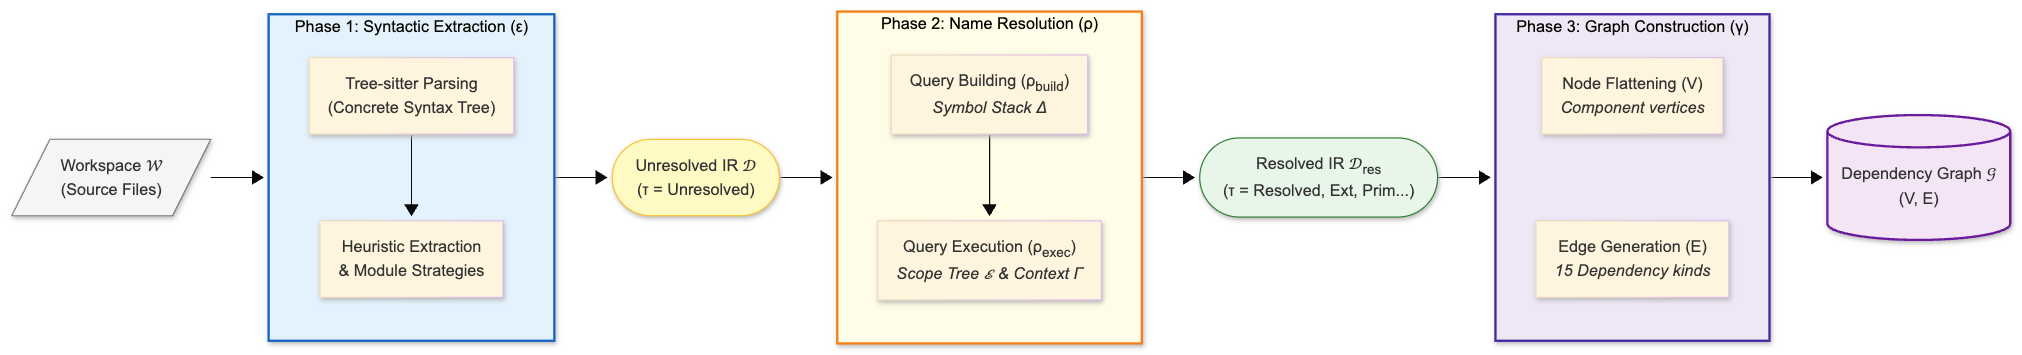
\includegraphics[width=\textwidth]{images/analysis_process/pipeline_detailed.png}
  \caption{Architectural overview of the three-phase analysis
    pipeline, from source
  code to dependency graph.}
  \label{fig:pipeline_detailed}
\end{figure}

A fundamental design property of this decomposition is the classical separation
between concrete syntax and semantic analysis, mirroring standard
compiler pipeline
architectures \cite{aho_compilers_2007}. Phase 1 is the only phase
that interacts
with language-specific syntax and parse trees. Phase 2 operates on
the uniform IR
and relies on the declarative language configuration $\mathcal{K}$ to
account for
language-specific semantic rules (such as scoping and import
visibility), inspired
by modular language product lines \cite{vacchi_neverlang_2015}. Finally, Phase 3
is purely structural and completely language-agnostic.

\section{Phase 1: Syntactic Extraction ($\varepsilon$)}
\label{sec:phase1_overview}

$$\varepsilon : \mathcal{W} \to \mathcal{D}$$

The extraction phase transforms source code into the Intermediate
Representation. For each source file in the workspace, a Tree-sitter
parser \cite{brunsfeld_treesitter_2018} generates a Concrete Syntax Tree
(CST), which is then traversed by a set of heuristic classifiers and
parsers to identify and extract the relevant software components
(modules, structured types, functions, fields, imports, and
implementation blocks).

\subsection{Input}

The input is a \textbf{Workspace} $\mathcal{W}$: a directory tree
containing source files in one or more of the supported languages (C,
C++, Java, Python, Rust). Each file is independently parsed and extracted.

\subsection{Process}

The extraction operates through four logical layers:

\begin{enumerate}
  \item \textbf{Parsing}: Tree-sitter generates a CST for each source
    file, preserving every token of the original code.
  \item \textbf{Classification}: Heuristic predicates inspect CST
    node kinds (e.g., \texttt{struct\_item},
    \texttt{function\_definition}, \texttt{class\_declaration}) using
    string-based pattern matching to determine the role of each node.
    This approach exploits the structural similarity of Tree-sitter
    grammars across languages to avoid maintaining per-language rule sets.
  \item \textbf{Structural Parsing}: Classified nodes are transformed
    into IR components by extracting their constituent parts (names,
    fields, methods, parameters, return types, super-types, annotations).
  \item \textbf{Body Extraction}: Function bodies are analyzed to
    extract behavioral dependencies (function calls, type
    instantiations, field accesses, type casts) and local variable
    declarations, organized into a recursive \texttt{Block} structure
    that mirrors the lexical scope hierarchy of the source code.
\end{enumerate}

After individual file extraction, a \textbf{Module Grouping Strategy}
organizes the extracted modules into a hierarchical tree that
reflects the project's namespace conventions. Different strategies
are applied depending on the language: directory-based namespacing
(Python, Rust), package declarations (Java), explicit namespace
blocks (C++), or a flat fallback (C). For C++, an additional
\textbf{out-of-line method linking} step associates method
definitions written in \texttt{.cpp} files with their class
declarations in \texttt{.hpp} headers.

\subsection{Output}

The output is a forest of \textbf{Module trees} $\vec{\mathcal{M}}
\in \mathcal{D}$,
unified across all files in the workspace. Each module contains its
structured types, free functions, imports, implementation blocks,
type aliases, and free variables. All type references ($\tau$) at
this stage are in their initial extraction states:
either raw symbolic identifiers $\text{Unresolved}(\pi_{\text{raw}})$
or composite
disjunctions $\text{Union}(\vec{\tau})$ for dynamic typing (e.g.,
Python type unions).
No cross-component linking or primitive matching has taken place yet.

\subsection{Key Properties}
\begin{itemize}
  \item This is the \textbf{only language-dependent} phase. The
    heuristic classifiers and extractors are the sole components that
    interact with language-specific CST node kinds.
  \item Each file is extracted \textbf{independently}. Cross-file
    dependencies are not resolved in this phase.
  \item The output IR is \textbf{structurally complete} but
    \textbf{semantically unresolved}: the topology of the codebase
    (what components exist and what they contain) is fully captured,
    but the targets of type references are not yet known.
\end{itemize}

The detailed implementation of this phase, including the heuristic
classification system, the extraction algorithms, and the module
grouping strategies, is presented in Chapter \ref{ch:extraction}.

\section{Phase 2: Name Resolution ($\rho$)}
\label{sec:phase2_overview}

$$\rho : \mathcal{D} \to \mathcal{D}_{\text{res}} \qquad \rho =
\rho_{\text{exec}} \circ \rho_{\text{build}}$$

The name resolution phase transforms the symbolic type references
produced by extraction into resolved semantic pointers. This is the
phase that connects the isolated components into a coherent
dependency network by determining, for each type reference, which
component in the workspace it refers to.

\subsection{Input}

The input is the forest of module trees $\vec{\mathcal{M}} \in \mathcal{D}$
produced by Phase 1, accompanied by the declarative Language Configuration
$\mathcal{K}$ and the Primitive Registry $\mathcal{P}$.

\subsection{Process}

The resolution is decomposed into two sequential steps:
$$\rho_{\text{build}} : \mathcal{D} \xrightarrow{\Delta}
\mathcal{D}_{\mathcal{Q}} \qquad \rho_{\text{exec}} :
\mathcal{D}_{\mathcal{Q}} \xrightarrow{\Gamma} \mathcal{D}_{\text{res}}$$

\begin{enumerate}
  \item \textbf{Query Building} ($\rho_{\text{build}}$): The module hierarchy
    is traversed with an ephemeral \textit{Symbol Stack} ($\Delta$)
    that tracks local variable bindings. Each \texttt{Unresolved}
    type reference is replaced by an algebraic \textit{Resolution
    Query} ($\mathcal{Q}$) composed of three primitives:
    \begin{itemize}
      \item \texttt{Find($s$)}: Ascending scope search for identifier $s$.
      \item \texttt{Extract($q$, $s$)}: Structural member access on
        the result of sub-query $q$.
      \item \texttt{Call($q$)}: Return-type extraction after
        evaluating sub-query $q$ as a callable.
    \end{itemize}
    The Symbol Stack enables local variable substitution: when a
    reference such as \texttt{x.method()} is encountered, the stack
    replaces \texttt{x} with its declared type, transforming the
    reference into a query that can be resolved globally.

  \item \textbf{Query Execution} ($\rho_{\text{exec}}$): A global \textit{Scope
    Tree} ($\mathcal{E}$) is constructed from the entire workspace
    using an arena allocator. Each query expression is then evaluated
    against this tree using \textit{Lexical Scope Climbing}: starting
    from the scope where the reference was declared, the algorithm
    ascends the parent chain, checking local symbols, imports, and
    inherited members, until the target is found or the root is reached.
\end{enumerate}

The resolution is parameterized by a per-language
\textbf{configuration} ($\mathcal{K}$) that controls behaviors
such as transitive import resolution, implicit self/this parameter
injection, and Deref coercion handling.

\subsection{Output}

The output of Phase 2 is the resolved forest of module trees
$\vec{\mathcal{M}}_{\text{res}} \in \mathcal{D}_{\text{res}}$, retaining the
isomorphic structural topology of the codebase while transforming every
raw identifier and deferred query expression into one of six post-resolution
states (as formalized in Figure \ref{fig:typeref_lifecycle} of
Chapter \ref{ch:ir_formalization}):

\begin{itemize}
  \item $\text{Resolved}(\pi_{\text{abs}})$: The reference was successfully
    bound to an internal component within the workspace, identified by its
    canonical absolute qualified name $\pi_{\text{abs}} \in \Pi$.
  \item $\text{External}(\pi_{\text{ext}})$: The reference points to an entity
    outside the analyzed workspace (e.g., standard library APIs, third-party
    packages or framework types), identified by its external qualified path
    $\pi_{\text{ext}} \in \Pi_{\text{ext}}$.
  \item $\text{Prim}(\iota_p)$: The reference denotes a fundamental built-in
    primitive type ($\iota_p \in \mathcal{P}$) registered in the
    language-specific Primitive Registry, requiring no namespace binding.
  \item $\text{Union}(\vec{\tau})$: A composite disjunctive type
    (such as dynamic type unions \texttt{Union[A, B]} in Python), where
    each constituent type reference $\tau_i \in \vec{\tau}$ has been
    recursively resolved.
  \item $\text{EvaluatedAccess}(\tau_{\text{path}}, \tau_{\text{type}})$: A
    compound resolution state resulting from field or member access chains,
    which retains both the evaluated receiver path $\tau_{\text{path}}$ and the
    terminal structural type $\tau_{\text{type}}$.
  \item $\text{Failed}(\pi_{\text{raw}})$: Static resolution was unable to
    locate the symbol in any accessible lexical, imported, or inherited scope,
    preserving the original unresolvable identifier
    $\pi_{\text{raw}}$ to support
    precision/recall metrics and fallback diagnostics.
\end{itemize}

\subsection{Key Properties}
\begin{itemize}
  \item This phase is \textbf{completely language-independent}. The
    resolution algorithm operates solely on the IR, with
    language-specific behavior controlled by configuration flags.
  \item The resolution is \textbf{workspace-global}: because the
    Scope Tree is built from all files simultaneously, cross-file
    dependencies are resolved transparently.
  \item The Execution Context ($\Gamma = \langle \mathcal{E},
    \mathcal{P}, \mathcal{K} \rangle$) is \textbf{immutable}
    during query evaluation, guaranteeing deterministic results
    independent of evaluation order.
\end{itemize}

The detailed implementation of this phase, including the query
algebra, the Scope Tree construction, the lexical climbing algorithm,
and the inheritance resolution mechanism, is presented in Chapter
\ref{ch:name_resolution}.

\section{Phase 3: Graph Construction ($\gamma$)}
\label{sec:phase3_overview}

$$\gamma : \mathcal{D}_{\text{res}} \to \mathcal{G}$$

The graph construction phase projects the resolved IR into a flat
directed dependency graph $\mathcal{G} = (V, E)$ suitable for
architectural analysis and visualization.

\subsection{Input}

The input is the resolved forest of module trees
$\vec{\mathcal{M}}_{\text{res}} \in \mathcal{D}_{\text{res}}$
produced by Phase 2, where type references populate their
post-resolution states.

\subsection{Process}

The construction proceeds in two steps:

\begin{enumerate}
  \item \textbf{Node Flattening}: The hierarchical module tree is
    recursively traversed, and every component (module, structured
    type, function, field, type alias) is extracted into a flat
    vector of vertices $V$. Each vertex receives a globally unique
    qualified name computed by prepending all ancestor module names.
    Additionally, implicit nodes are synthesized for primitive types
    and external dependencies that are referenced by edges but not
    declared in the workspace.
  \item \textbf{Edge Generation}: The module tree is traversed a
    second time, inspecting every resolved type reference to emit
    directed edges. The system defines 15 distinct edge kinds
    organized into five categories: structural (containment and
    nesting), inheritance, type-level (field types, parameter types,
    return types), behavioral (calls, instantiations, field
    accesses), and auxiliary (imports, casts, annotations). After
    generation, edges are deduplicated to prevent inflated coupling metrics.
\end{enumerate}

The graph is exported in two formats: a raw JSON serialization of the
full \texttt{DependencyGraph} structure, and a
Cytoscape.js-compatible format \cite{franz_cytoscapejs_2016} where
structural containment is encoded as compound node nesting rather
than explicit edges.

\subsection{Output}

The output of Phase 3 is a unified \textbf{Dependency Graph}
$\mathcal{G} = (V, E)$:
\begin{itemize}
  \item $V$: A set of component vertices $v \in \mathcal{C}$, each
    identified by its
    canonical qualified name $\pi(v) \in \Pi$ and typed by its
    architectural kind
    (Module, Structured Type, Function, Field, Type Alias, Primitive, External).
  \item $E$: A set of directed dependency edges $E \subseteq V \times
    V \times \mathcal{K}_{\text{edge}}$,
    where each directed edge $e = \langle u, v, k \rangle$ specifies
    the source component $u$,
    the target component $v$, and the taxonomic dependency kind $k
    \in \mathcal{K}_{\text{edge}}$.
\end{itemize}

An \texttt{AnalysisSummary} is also produced, containing aggregate
statistics (total modules, structured types, free functions, resolved
references, and failed references).

\subsection{Key Properties}
\begin{itemize}
  \item This phase is \textbf{completely language-independent}. The lowering
    algorithm operates uniformly over the resolved IR without
    language-specific branches.
  \item \textbf{Comprehensive Target Extraction}: Dependency edges
    are emitted from all
    semantically meaningful type references. While $\text{Resolved}$
    and $\text{External}$
    produce direct dependency targets, $\text{Primitive}$ references
    generate edges to
    synthesized primitive nodes, $\text{Union}(\vec{\tau})$
    references recursively decompose
    into edges toward all constituent types, and
    $\text{EvaluatedAccess}$ references produce
    edges to both the accessed receiver and the resulting type.
    Failed references do not emit
    spurious edges, avoiding noise in coupling metrics.
  \item \textbf{Graph Closure Property}: The constructed graph is
    strictly closed:
    $\forall \langle u, v, k \rangle \in E \implies u \in V \land v \in V$.
    Whenever a resolved reference targets an external library or a
    primitive type
    not present among declared workspace entities, synthetic vertices
    (\texttt{Component::External} and \texttt{Component::Primitive})
    are dynamically
    instantiated in $V$ to guarantee structural integrity.
  \item The graph is \textbf{flat}: the original hierarchical nesting
    is encoded either as explicit containment edges or, in the
    Cytoscape export, as compound node parent relationships.
\end{itemize}

The detailed implementation of this phase, including the flattening
algorithm, the complete edge taxonomy, and the Cytoscape export
process, is presented in Chapter \ref{ch:graph_construction}.

\section{End-to-End Data Flow}
\label{sec:data_flow}

Table \ref{tab:pipeline_summary} summarizes the domain transformations,
operational contexts, and characteristics of each phase across the pipeline.

\begin{table}[htpb]
  \centering
  \small
  \begin{tabular}{|l|c|l|l|l|l|}
    \hline
    \textbf{Phase} & \textbf{Op.} & \textbf{Input Domain} &
    \textbf{Output Domain} & \textbf{Context} & \textbf{Scope} \\ \hline
    1. Extraction & $\varepsilon$ & Source files $\mathcal{W}$ &
    Unresolved IR $\mathcal{D}$ & Tree-sitter CST & Per-file \\ \hline
    2a. Query Building & $\rho_{\text{build}}$ & Unresolved IR
    $\mathcal{D}$ & Query IR $\mathcal{D}_{\mathcal{Q}}$ & Symbol
    Stack $\Delta$ & Local scope \\ \hline
    2b. Query Execution & $\rho_{\text{exec}}$ & Query IR
    $\mathcal{D}_{\mathcal{Q}}$ & Resolved IR
    $\mathcal{D}_{\text{res}}$ & Context $\Gamma = \langle
    \mathcal{E}, \mathcal{P}, \mathcal{K} \rangle$ & Workspace-wide \\ \hline
    3. Graph Construction & $\gamma$ & Resolved IR
    $\mathcal{D}_{\text{res}}$ & Dependency Graph $\mathcal{G}$ &
    Registry $\mathcal{P}$ & Workspace-wide \\ \hline
  \end{tabular}
  \caption{Summary of the pipeline transformations: operators,
  domains, operational contexts, and scope.}
  \label{tab:pipeline_summary}
\end{table}

This pipeline architecture establishes several key guarantees:
\begin{enumerate}
  \item \textbf{Type-Safe Functional Composition}: Each stage is a
    pure deterministic
    function over well-defined domains \cite{pierce_types_2002}. The
    end-to-end transformation
    $\phi = \gamma \circ (\rho_{\text{exec}} \circ
    \rho_{\text{build}}) \circ \varepsilon$
    is well-typed and preserves structural correctness across lowering steps.
  \item \textbf{Determinism and Confluence}: Because the execution context
    $\Gamma = \langle \mathcal{E}, \mathcal{P}, \mathcal{K} \rangle$
    remains immutable
    during query evaluation, query evaluation has no side effects on
    the environment.
    Consequently, evaluating type queries in any order yields identical results.
  \item \textbf{Guaranteed Termination}: The pipeline terminates for
    any finite workspace:
    the CST traversal is bounded by the finite node depth of parse
    trees, lexical scope climbing
    is bounded by the finite height of the Scope Tree $\mathcal{E}$,
    and inheritance resolution
    employs cycle detection to prevent infinite loops.
  \item \textbf{Graph Closure}: As established in Section
    \ref{sec:phase3_overview},
    Phase 3 ensures that $\forall \langle u, v, k \rangle \in E
    \implies u \in V \land v \in V$.
    Synthetic vertices are dynamically added to $V$ for primitive
    types and external libraries,
    guaranteeing that the exported graph contains no dangling edges.
  \item \textbf{Extensibility}: Adding support for a new language
    requires implementing
    only the syntactic CST extraction (Phase 1) and declaring its
    configuration $\mathcal{K}$
    (Phase 2). The query algebra, scope climbing, and graph
    construction remain entirely reused.
\end{enumerate}
